\documentclass[12pt]{article}

\usepackage[utf8]{inputenc}
\usepackage[T1]{fontenc}
\usepackage{graphicx}

\title{A* dla układanki "15"}
\author{Nel Skowronek}
\date{}

\begin{document}

\maketitle

\section{Heurystyki}

\subsection{Manhattan Distance + Linear Conflict}

Z drobną modyfikacją: pogorszyłam Linear Conflict, żeby heurystyka była monotoniczna. 
Zamiast zliczać wszystkie konflikty występujące w danym rzędzie / danej kolumnie, zliczam 
tylko te, które się "widzą" (\textit{break} po znalezieniu konfliktu).

\subsection*{Przykład działania}

Dla rzędu pierwszego od góry takiego stanu: \\ \\
\begin{tabular}{|c|c|c|c|}
\hline
4 & 3 & 8 & 1 \\
\hline
13 & 0 & 7 & 2 \\
\hline
11 & 6 & 9 & 10 \\
\hline
12 & 14 & 15 & 5 \\
\hline
\end{tabular} \\ \\
Klasyczny linear conflict: \textbf{+6} ((4, 3), (4, 1), (3, 1)) \\ 
Mój linear conflict: \textbf{+4} ((4, 3), (3, 1)) \\

\subsection*{Monotoniczność - dowód}

Największym problemem klasycznego Linear Conflict są sytuacje, w których mamy element po srodku wiersza 
(odpowiednio: kolumny) konfliktujący z przynajmniej dwoma elementami po obydwu jego stronach. 
- W powyższym przykładzie jest to \textbf{3}, która konfliktuje z \textbf{4} po lewej i \textbf{1} po prawej. 
- Powoduje to, że przy przesunięciu tego elementu poza wiersz (zamiana \textbf{3} z \textbf{0}) 
"znikają" nam aż dwa konflikty, każdy liczony po \textbf{+2}. Przy jednoczesnym wzroście Manhattan Distance o \textbf{+1}, 
w sumie wartość oceny heurystycznej zmalała nam o \textbf{-3} względem poprzedniego stanu. \\

Aby to naprawić (pozwalać na spadek maksymalnie \textbf{-1}), korzystam z tego, że konflikty są przechodnie. 
T.j. jeśli w naszym przykładzie \textbf{3} konfliktuje z \textbf{4} po lewej i \textbf{1} po prawej - to \textbf{4} 
konfliktuje z \textbf{1}. \\

Manhattan Distance jest heurystyką monotoniczną, sytuacja w której element przed przesunięciem ma tylko jeden konflikt 
też jest trywialna, a więc jedynym momentem gdzie potencjalnie możemy mieć większy spadek oceny heurystycznej jest taki, jak 
ten opisany powyżej: element jest po środku dwóch konfliktów. \\

W takiej sytuacji, w momencie kiedy przesuwamy środkowy element poza rząd tracimy 2 konflikty (ponieważ zliczamy tylko "widzące się"), 
ale jednocześnie z przechodniości wynika, że zyskujemy 1 nowy konflikt. Ponieważ środkowy element został odsunięty od swojego 
rzędu docelowego, Manhattan Distance wzrośnie o \textbf{+1}. W sumie dając nam maksymalny spadek oceny heurystycznej równy \textbf{-1} 
względem poprzedniego stanu. \\

A więc mój zmodyfikowany Linear Coflict jest monotoniczny.

\subsection{Walking Distance}

Znana, monotoniczna heurystyka, tym razem bez żadnych modyfikacji. Zlicza liczbę kroków, potrzebną do przesunięcia stanu, 
w którym wszystkie elementy są w odpowiadającym im docelowych rzędach / kolumnach, do dowolnego innego stanu, nierozróżniając 
poszczególnych elementów, tylko skupiając się na ich rzędach docelowych. \\

W celu wyliczenia Walking Distance, zrobiłam precomputing polegający na:
\begin{enumerate}
    \item Rozpoczęciu od stanu:
        \begin{tabular}{|c|c|c|c|c|}
        \hline
         & A & B & C & D \\
        \hline
        A & 4 & 0 & 0 & 0 \\
        \hline
        B & 0 & 4 & 0 & 0 \\
        \hline
        C & 0 & 0 & 4 & 0 \\
        \hline
        D & 0 & 0 & 0 & 3 \\
        \hline
        \end{tabular}
    \item Wyliczeniu sąsiadujących stanów
    \item Dodawaniu sąsiednich stanów do kolejki przeszukiwania i zapisywaniu ich wraz z obecną odległością
    \item Powtarzaniu, aż nie zostaną przeszukane wszystkie stany
    \item Zapisaniu do bazy danych (pliku binarnego)
\end{enumerate}
Zauważyłam, że sytuacja dla rzędów i kolumn jest symetryczna, więc precomputing zrobiłam tylko dla rzędów, a w A\* obliczam stan 
rzędów i kolumn analogicznie i wyszukuję w bazie danych Walking Distance.

\section{Generowanie Permutacji}

Do generowania permutacji w C++ używam standardowej funkcji \textbf{std::shuffle}. Według dokumentacji generuje permutacje 
z rozkładu jednostajnego.

\section{Działanie}

Dla maksymalizacji efektywności stany planszy przechowuję w liczbach 64 bitowych, a większość operacji używanych m.in. przy wyznaczaniu 
sąsiadów to operacje bitowe (głównie bitshifty, koniunkcje i alternatywy). Surowe stany opakowuję w obiekty \textbf{Node} trzymające informacje 
o własnych wartościach g(), h() i f(), oraz wskaźnik (32 bity) na Node, z którego "przyszedł", co potem bardzo ułatwia śledzenie ścieżki. 
Node'y do odwiedzenia przetrzymuję w kolejce priorytetowej (insert / pop = O(log n), ocenia priorytet po wartościach f()), a odwiedzone 
w hash-mapie (insert / find = O(1)).

\section{Wykresy}

\begin{figure}[h]
    \centering
    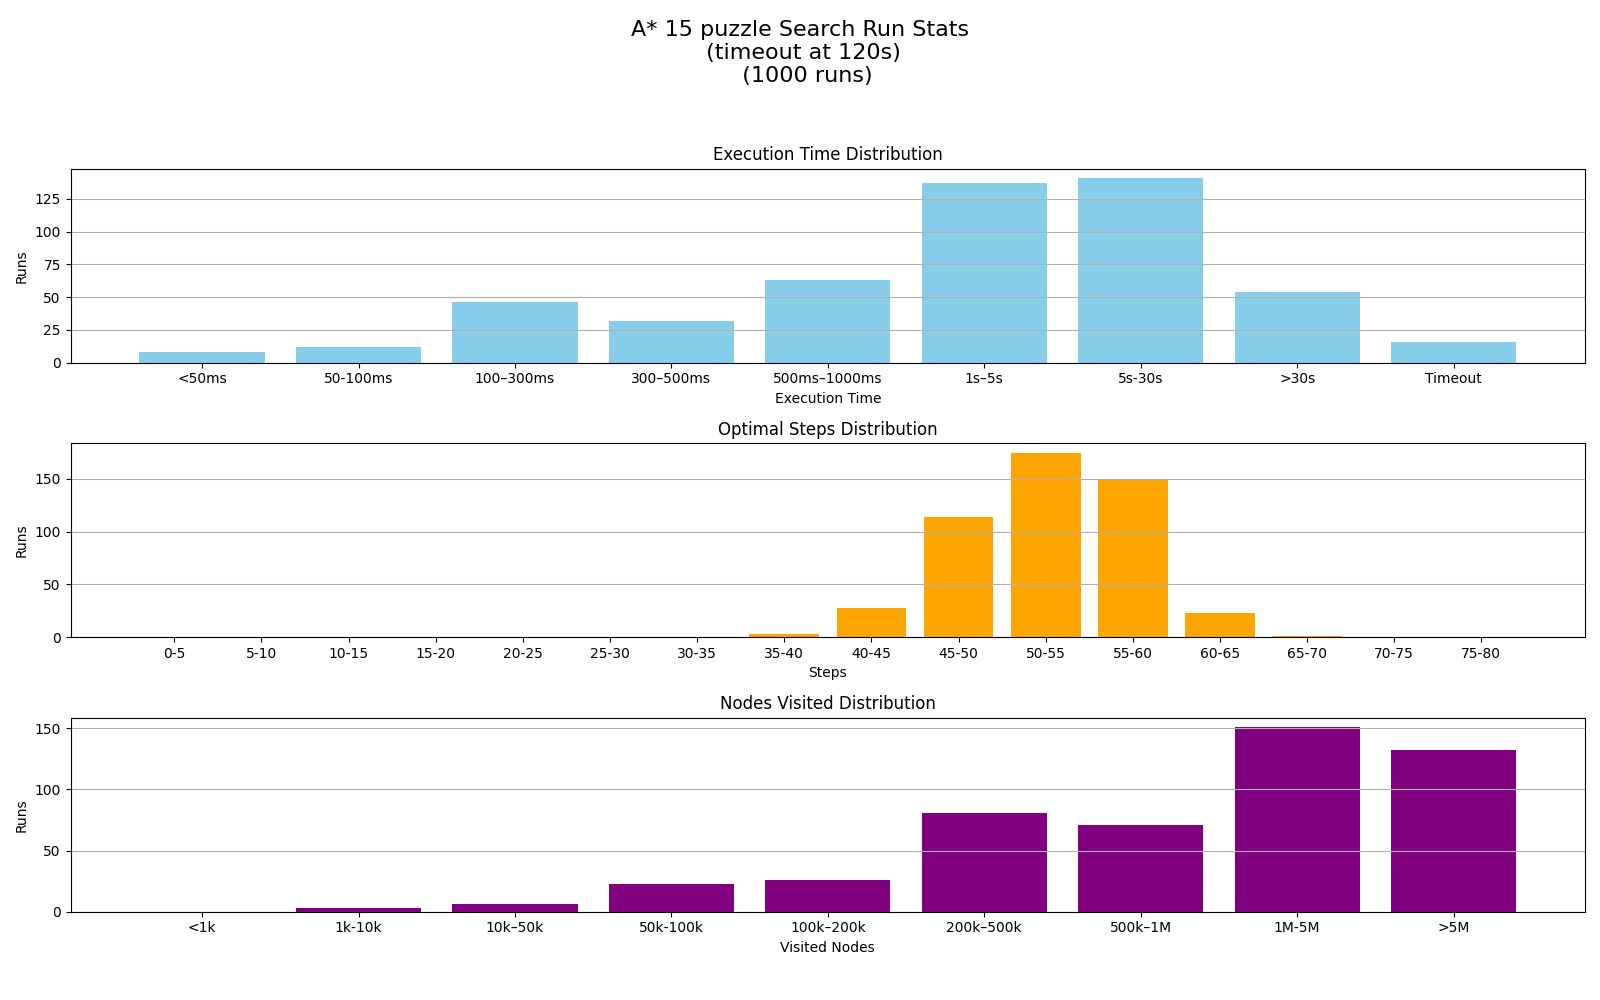
\includegraphics[width=\textwidth]{plots/(MDLC)aStar_run_stats_1000_runs.png}
    \caption{Statystyki dla Manhattan Distance + Linear Conflict}
    \label{fig:sample}
\end{figure}

\begin{figure}[h]
    \centering
    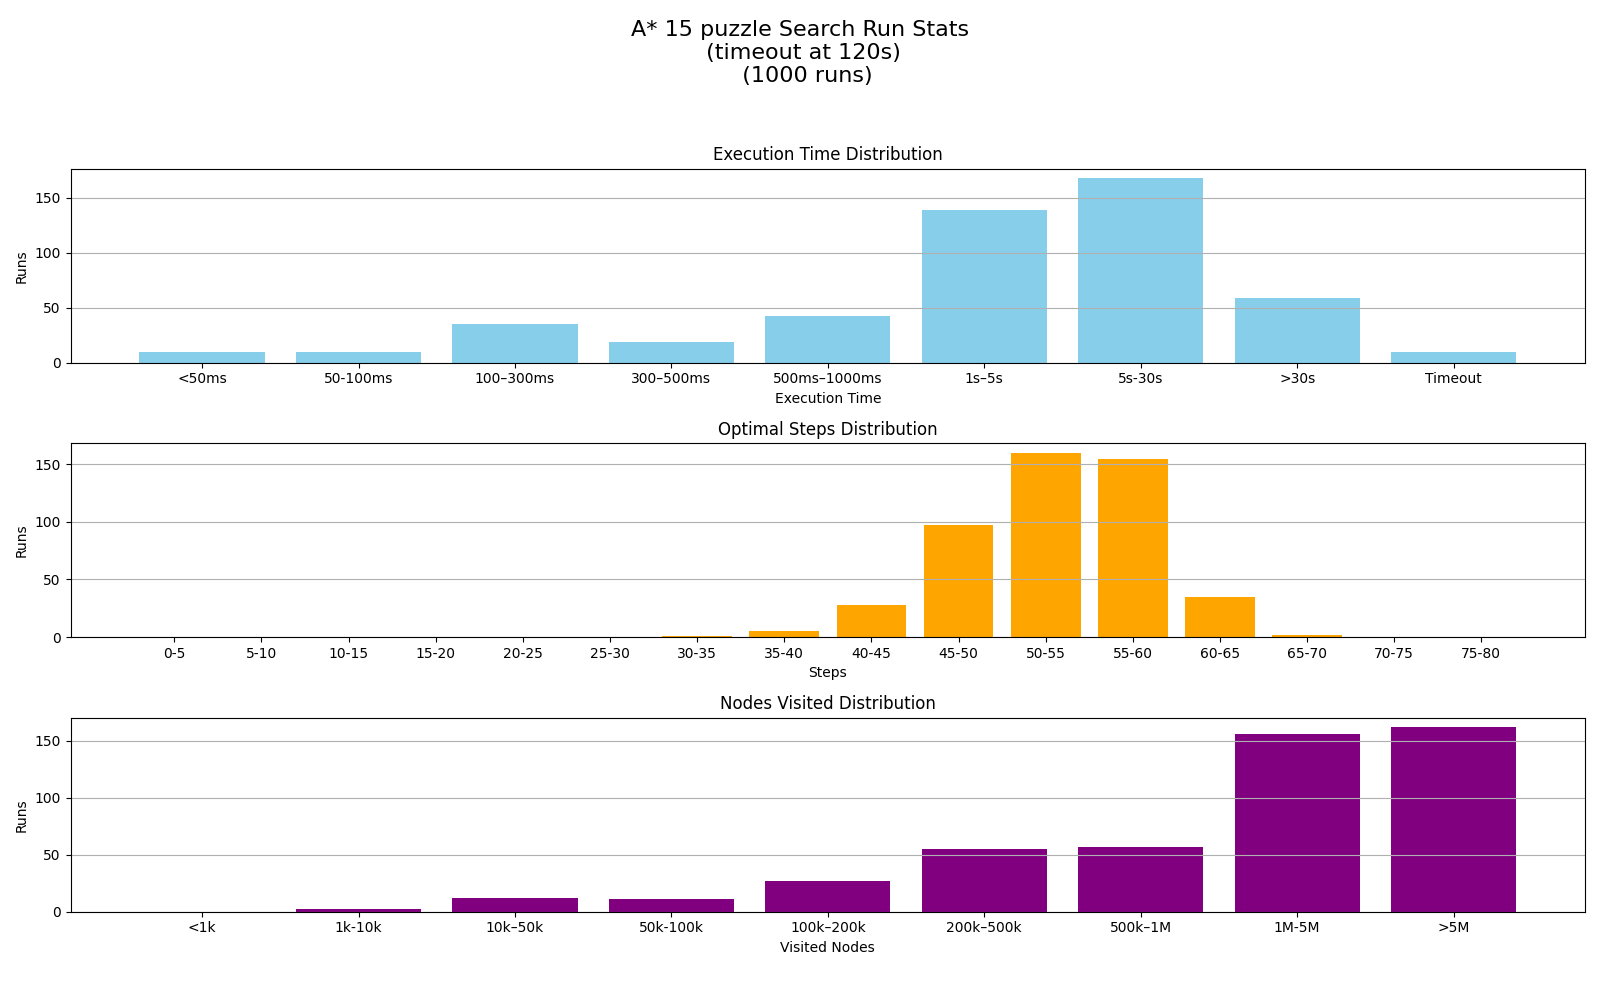
\includegraphics[width=\textwidth]{plots/(WD)aStar_run_stats_1000_runs.png}
    \caption{Statystyki dla Walking Distance}
    \label{fig:sample}
\end{figure}

\begin{figure}[h]
    \centering
    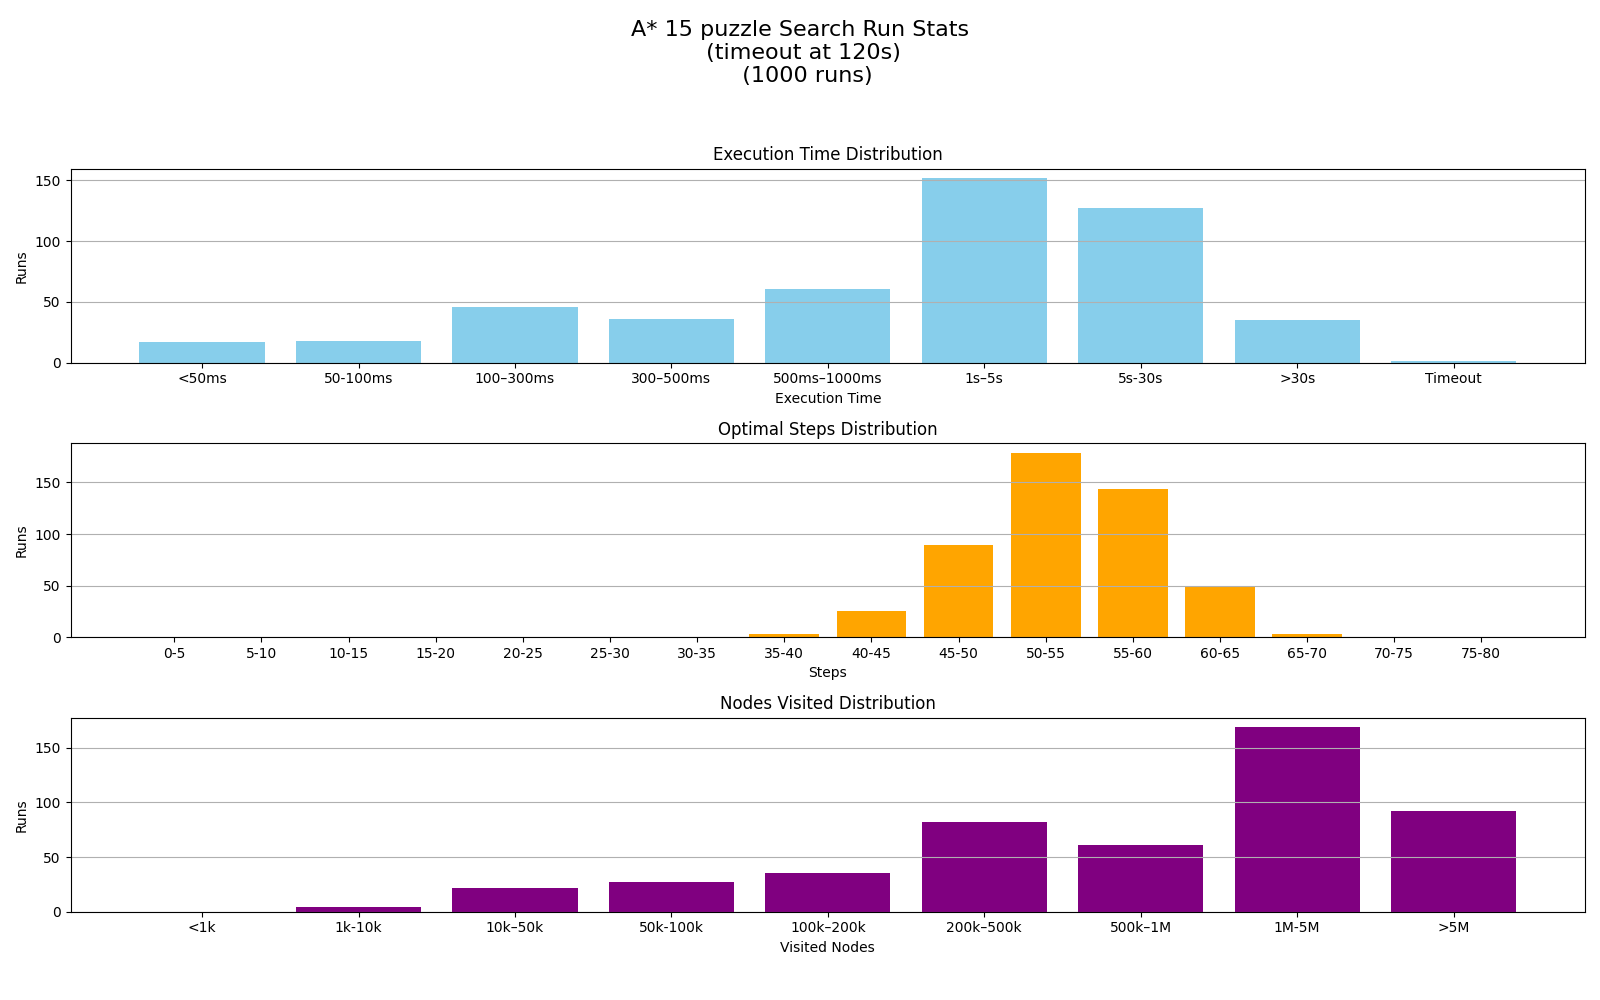
\includegraphics[width=\textwidth]{plots/(MAX)aStar_run_stats_1000_runs.png}
    \caption{Statystyki dla maksimum z obu heurystyk (najlepsza)}
    \label{fig:sample}
\end{figure}

\end{document}